% !TEX TS-program = xelatex
% !TEX encoding = UTF-8 Unicode
% !Mode:: "TeX:UTF-8"

\documentclass{resume}
\usepackage{zh_CN-Adobefonts_external} % Simplified Chinese Support with automatic font fallback
% \usepackage{NotoSansSC_external}
% \usepackage{NotoSerifCJKsc_external}
% \usepackage{zh_CN-Adobefonts_internal} % Simplified Chinese Support using system fonts
\usepackage{array}
\usepackage{graphicx}
\usepackage{setspace} % provides onehalfspacing environment
\usepackage{cite}

\begin{document}
\pagenumbering{gobble} % suppress displaying page number

\name{AI产品方向简历}

\basicInfo{
  \email{zhoulukai329@gmail.com} \textperiodcentered\
  \phone{(+86) 189-3991-4215} \textperiodcentered\
  \github{https://github.com/zhoulukai329-spec}
}

\section{\texorpdfstring{{\normalfont\faInfo}\ }{}个人概况}

\noindent
\begin{minipage}[t]{0.80\textwidth}
\vspace{0pt}
\small
\begin{spacing}{1.04}
\addfontfeatures{LetterSpace=0.8}
\setlength{\tabcolsep}{0pt}
\renewcommand{\arraystretch}{1.05}
\begin{tabular}{@{}>{\raggedright\arraybackslash}p{0.19\linewidth}@{\hspace{0.7em}}>{\raggedright\arraybackslash}p{0.77\linewidth}@{}}
姓名： & 周路凯 \\
性别： & 男 \\
出生日期： & 2006年3月29日 \\
学历： & 本科（2028届） \\
专业： & 网络空间安全 \\
联系电话/微信： & +86 18939914215（微信号: zlk94hhz） \\
AI使用情况： & 熟悉主流大语言模型，熟悉大部分热门开源模型的使用场景；\\ 
&具备大模型实际接入经验，能够通过 API 调用模型完成自建 Agent 推理，也尝试过从 Huggingface 部署开源模型并接入 AI Agent 进行实际使用；\\ 
&日常使用 Codex、Trae 等 Agent 产品辅助开发、调试与问题分析；\\ 
& 有Prompt Engineering 经验，能够保证Prompt的规范性，符合Role机制等主流的输入方法。\\

\end{tabular}
\end{spacing}
\end{minipage}\hfill
\begin{minipage}[t]{0.16\textwidth}
\vspace{0pt}
\raggedleft
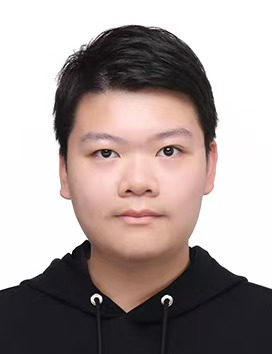
\includegraphics[width=\linewidth,height=0.18\textheight,keepaspectratio]{photo.jpg}
\end{minipage}


\section{\texorpdfstring{{\normalfont\faGraduationCap}\ }{}教育背景}
\datedsubsection{\textbf{厦门大学}}{2024年9月 -- 至今}
\textit{本科}\ 网络空间安全, 预计 2028 年 6 月毕业\\
相关课程及表现: 人工智能原理(未出分) , 计算机网络(未出分) , 操作系统原理(未出分) , C语言程序设计(A) , 算法设计与分析(A) , 概率论与统计(A) , 数据库原理(B+) , 选修: AI智能体与工作流自动化(B+)

\section{\texorpdfstring{{\normalfont\faUsers}\ }{}项目经历}
\datedsubsection{\textbf{基于 LangChain 架构的 AI Agent 数据库去重项目}}{2026年3月 -- 2026年5月}
\role{Python, LangChain}{团体项目实践（与企业 BlackBerry 合作项目）}
面向脱敏业务数据，设计并实现基于 LangChain 架构的 AI Agent 数据库去重项目\\ 
\begin{onehalfspacing}
https://github.com/Fovir-GitHub/ccoe\\
主要贡献：
\begin{projectitems}
  \item 设计并实现基于 AI Agent 的数据库去重与效果评估流程
  \item 利用 LangChain 架构，实现 AI Agent 的推理
  \item 基于 Python 进行数据预处理和标准化, 调用 API （或通过Ollama等渠道加载本地模型）进行 Embedding 生成向量, 再将此步骤打包为 Tool 供agent自行使用, 之后接入 AI Agent 自行使用tool进行数据处理, 并进行相似度计算
  \item 基于姓名、邮箱、公司、课程等字段构建标准化指纹生成逻辑，对原始数据集与去重结果集进行比对，建立 TP、FP、TN、FN 四类离线评估体系
  \item 设计 0.85--0.95 阈值敏感性实验，分析 Precision 与 Recall 的变化趋势，定位最优阈值区间为 [0.88, 0.92]，为平衡误删与漏检提供参数依据
  \item 在最优阈值 0.90 下实现 Precision 约 0.83、Recall 约 0.92; 同时识别脱敏测试数据导致核心特征受限的问题，提出生产环境下的特征重构与策略迭代方向
\end{projectitems}
\end{onehalfspacing}
\projectdivider

\datedsubsection{\textbf{面向复杂规则任务的 AI Agent 与强化学习系统}}{2026年6月 -- 至今}
\role{Python, Reinforcement Learning, CNN, ReAct}{合作项目}
面向带有复杂且未知规则的不同小游戏，设计并实现具备感知、决策、执行与反馈闭环以适应规则自主通关的 AI Agent 系统\\
https://github.com/zhoulukai329-spec/arc-intelligence-agent.git (由于相关比赛的开展，本项目尚未开源，等相关比赛结束再开源)\\
主要贡献:
\begin{onehalfspacing}
\begin{projectitems}
  \item 设计并落地 ``环境适配 + 特征提取 + 策略学习 + 训练评估'' 的强化学习主链路，完成从状态到动作决策的闭环建模
  \item 基于颜色分布、质心位置、动作掩码、进度比率与帧间变化等信号构建通用状态特征，支撑跨任务共享策略学习
  \item 实现轻量级 Policy Gradient 风格训练框架，包含训练/验证拆分、epsilon-greedy 探索、折扣回报更新与 advantage 优化
  \item 设计 ``眼睛-大脑-手'' 分层协作架构，将感知编码、规则推理、动作规划、执行校验与记忆模块解耦，提升系统可扩展性与可解释性
  \item 构建奖励机制与离线评测流程并不断微调参数，通过步长惩罚、进度奖励、重复状态惩罚和终局奖励优化 agent 行为质量与泛化能力
\end{projectitems}
\end{onehalfspacing}
\projectdivider

\datedsubsection{\textbf{基于 神经网络、强化学习和 PPO优化策略的五子棋对战游戏}}{2026年5月 -- 2026年6月}
\role{Python, PyTorch, RL, CNN, PPO}{个人项目}
\begin{onehalfspacing}
五子棋智能对战游戏, https://github.com/zhoulukai329-spec/Gomoku\_Master\_for\_SOF106
\begin{projectitems}
  \item 基于 PyTorch 实现五子棋 PPO Actor-Critic 智能体，采用 3 通道棋盘编码、残差 CNN 特征提取和 Policy/Value 双头网络，支持 15x15 棋局状态建模与落子决策
  \item 设计自博弈训练流水线，引入合法落子 masking、开局/残局温度控制、奖励塑形、梯度裁剪与 best checkpoint 对战评估，提升策略训练的稳定性与迭代效率
  \item 开发 Pygame 人机对战界面，并集成必胜/必防战术启发、自动 bootstrap 训练、权重加载和 PyInstaller 单文件打包发布流程，支持训练、推理与可执行程序分发
\end{projectitems}
\end{onehalfspacing}


% Reference Test
%\datedsubsection{\textbf{Paper Title\cite{zaharia2012resilient}}}{May. 2015}
%An xxx optimized for xxx\cite{verma2015large}
%\begin{itemize}
%  \item main contribution
%\end{itemize}

\section{\texorpdfstring{{\normalfont\faCogs}\ }{}技术栈}
% increase linespacing [parsep=0.5ex]
\begin{itemize}[parsep=0.5ex]
  \item 编程语言: Python, C/C++, Golang, mySQL, Java
  \item 操作系统: Windows, Linux
  \item 框架: PyTorch, LangChain等
  \item 版本控制: Git, GitHub
  \item 容器化: Docker
  \item 产品能力: PRD
\end{itemize}

\section{\texorpdfstring{{\normalfont\faHeartO}\ }{}获奖情况}
\datedline{美国大学生数学建模大赛, \textit{Finalist 特等奖提名}}{2026年2月}
\datedline{全国大学生创新创业大赛, \textit{省二等奖}}{2025年7月}

\section{\texorpdfstring{{\normalfont\faInfo}\ }{}其他}
% increase linespacing [parsep=0.5ex]
\begin{itemize}[parsep=0.5ex]
  \item GitHub: https://github.com/zhoulukai329-spec
  \item 语言: 英语 - 熟练(本科阶段有海外留学经历)
\end{itemize}

%% Reference
%\newpage
%\bibliographystyle{IEEETran}
%\bibliography{mycite}
\end{document}
